\documentclass[10pt]{article}
\usepackage[utf8]{inputenc}
\usepackage{parskip}
\usepackage[a4paper, margin=1.5in]{geometry}
\usepackage{graphicx}
\usepackage{hyperref}
\usepackage{listings}
\usepackage{array}

\renewcommand{\arraystretch}{1.5}

\title{Task 1 Report}
\date{11/11/2019}
\author{Federico Fregosi, Mirko Laruina,\\
        Riccardo Mancini, Gianmarco Petrelli}

\begin{document}
\pagenumbering{gobble}
\maketitle
\vfill
% \setcounter{tocdepth}{1}
\tableofcontents
\vfill
\clearpage
\setcounter{page}{1}
\pagenumbering{arabic}

\section{Specifications}
\subsection{Application overview}
The application is a messaging system where registered users can create an 
account, exchange text messages and make groups.

A registered user can initiate a chat with another user, create a new group chat
(of which he becomes the admin) and send messages to the chats he belongs to,
as well as receiving messages from those chats. He can also leave a group.

A group admin can add and remove new users to the group. He cannot assign his
powers to another user in the group and if he leaves the group, the latter 
is deleted.

Everytime a user views a chat, all the latest messages from the chat are fetched from 
the server and shown to the user.

\subsection{Actors}
Anonymous user, registered user, group admin and a time-based event.

\subsection{Functional specifications}

An \textbf{anonymous user} must be able to register in order to become a 
\emph{registered user}.

A \textbf{registered user} must be able to:
\begin{itemize}
    \item Send a message to a chat
    \item Read chat messages
    \item Create a private chat
    \item Create a group chat
\end{itemize}

A \textbf{group admin} must be able to:
\begin{itemize}
    \item Add users to the group
    \item Remove users from the group
\end{itemize}

The \textbf{time-based event} updates the user interface on regular intervals
to show new received messages from the current chat, if any.

\subsection{Software Architecture}
The proposed software architecture is a classic three-layer architecture:
\begin{enumerate}
    \item database (MySQL)
    \item server back-end (Java + Spring)
    \item user web app (ReactJS)
\end{enumerate}

\clearpage
\section{Analysis}
\subsection{Use-case diagram}
\begin{figure}[h!]
    \centering
    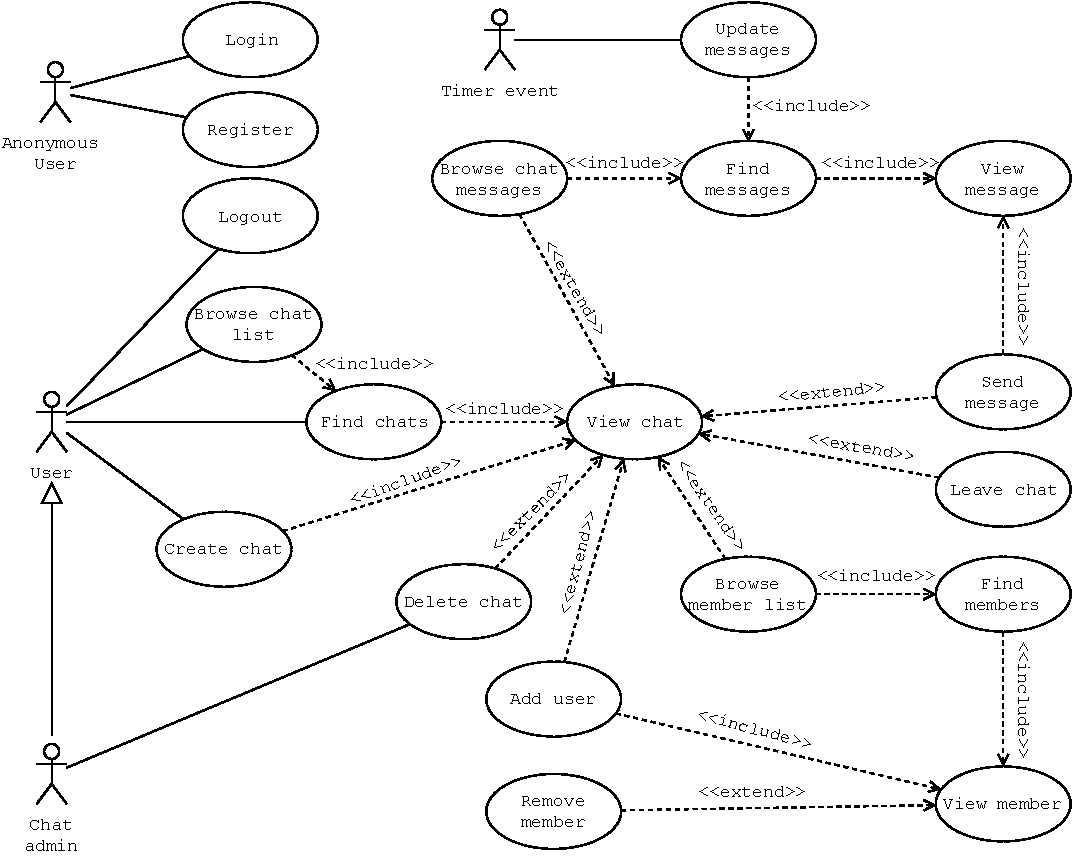
\includegraphics[width=\textwidth]{figs/use_case_diagram}
    \caption{Use-case diagram}
    \label{fig:usecase}
\end{figure}
Figure~\ref{fig:usecase} shows the use-case diagram for the project. Please note 
that the \texttt{Add user} and \texttt{Remove member} 
operations are only allowed to the \texttt{Chat admin}.

\subsection{Class diagram}
\begin{figure}[h!]
    \centering
    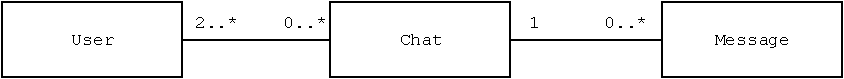
\includegraphics[width=\textwidth]{figs/class_diagram}
    \caption{Class diagram for the identified entities.}
    \label{fig:class_diagram}
\end{figure}

Figure~\ref{fig:class_diagram} shows the class diagram derived from the specifications. 
It can be seen that we chose to keep it as simple as possible by not making  
any distinction between \emph{private chats} and \emph{group chats}, 
creating a single \emph{Chat} entity.

\clearpage
\section{Implementation}

\subsection{Java backend}
The Java backend provides simple REST APIs for managing the chat application. 
In order to do so, it uses the \emph{Spring} framework\footnote{More information
at \url{https://spring.io/}}.
The list of the APIs and their description can be found in the 
\texttt{docs/api.md} file. The APIs return a JSON document, generated using
\emph{Google GSON}\footnote{More information at 
\url{https://github.com/google/gson}}, which is interpreted and shown to the user
by the ReactJS frontend.
These APIs are implemented using a simple database abstraction layer which provides 
corresponding APIs to the database. This is implemented in Java 
using a generic \emph{DatabaseAdapter} interface that can be implemented to 
provide access to different databases (as we have done in this Task with plain SQL, 
JPA and levelDB implementations). The database backend can be set from a configuration
file, where some other db-specific settings can be set.

The database APIs have been tested using some test units through \emph{JUnit4}
\footnote{More information at \url{https://junit.org/junit4/}} before being 
integrated with the ReactJS frontend.

\subsection{ReactJS frontend}
The fronted has been developed using the \emph{ReactJS} framework\footnote{More
information at \url{https://reactjs.org/}}. An overview of the main functions 
is available in the user guide (\texttt{docs/user\_guide/user\_guide.pdf}).

Regarding the implementation, the most notable thing is the timer-based event
that updates the UI. In particular, the client makes a request to the server
every second for updating the list of chats and every half second for updating 
the list of messages in the current chat.

\subsection{Limitations}
\paragraph{Passwords}
For the sake of simplicity, password hashing has not been implemented into the 
application. However, this could be simply integrated with a future update.

\paragraph{Polling}
In the current implementation, the server is polled every second for updating 
the list of chats and every half second for updating the list of messages. This 
is indeed a great load on the server in case there are many clients connected 
at the same moment. 
This problem has been alleviated by requesting only a subset of the chat 
messages, based on the timestamp on the latest received message.
However, 
a more appropriate way to handle it would be having a kind of notification API
that can be ``long polled''\footnote{A ``long poll'' is when the client 
makes a request to the server and the server does not respond until new 
information is available, at the cost of timing out the connection, at which 
point a new request is made.} by the client.

\section{Database}
\subsection{MySQL}
\begin{figure}[]
    \centering
    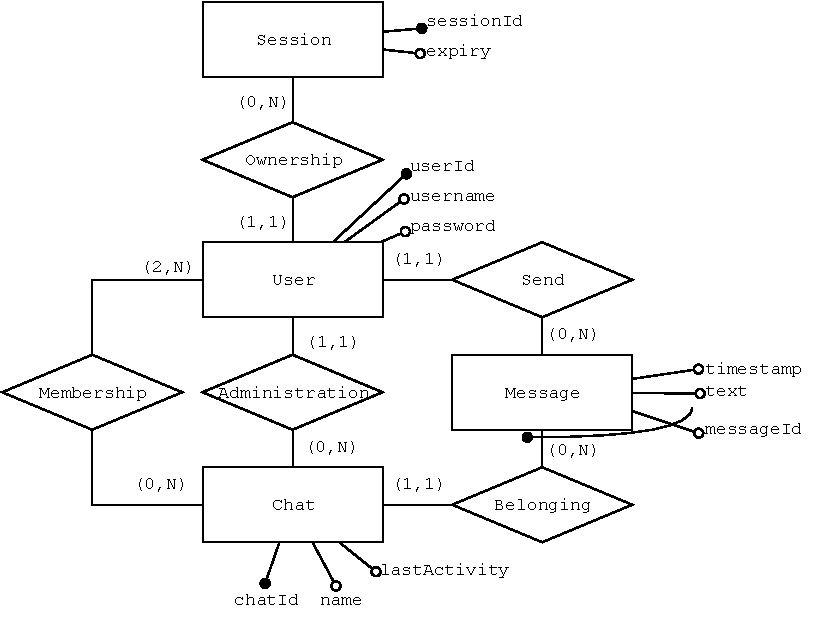
\includegraphics[width=\textwidth]{figs/ER}
    \caption{ER diagram for the database.}
    \label{fig:er}
\end{figure}

Figure~\ref{fig:er} shows the ER diagram of the MySQL database. Every \emph{User} 
is identified a \emph{userId} and has got a unique \emph{username} and a 
\emph{password}. The user can be a member of many \emph{Chats} and can 
be the administrator of many \emph{Chats}. On the other hand, a \emph{Chat} 
can be administered by only one \emph{User}. A \emph{User} can send a 
\emph{Message} to a \emph{Chat}. Each \emph{User} and each \emph{Chat} can 
have many \emph{Messages} while a \emph{Message} can belong to one \emph{Chat}
and one \emph{User} only. The \emph{Session} represents a logged user session.
Each \emph{User} can have many open \emph{Sessions}.

Once the database had been created, we filled it with random test data using the free
service available at \url{http://filldb.info/}. Generated data is not perfect, 
since some more complex functional constraints could not be included in the 
generation. However, that was sufficient for the first functional tests of the
application.

\subsubsection{JPA}
Given the database, the Java implementation using JPA was very fast, especially
compared to using plain SQL. We made use of both one-to-many and many-to-many 
relationships as it can be seen from the ER diagram.

\subsection{Key-Value}
\subsubsection{Feasability study}
\paragraph{Naive design}
Starting from the entity model and the use-cases, we first drafted a naive key-value 
implementation for the database and then we checked againts the use-cases whether 
it was efficient and we made some tweaks to it in order to improve it. 

We decided to generate ids incrementally by saving in the database the next id
to be generated. This value will be updated anytime a new element is generated.

Another design choice we made is to represent the many to many relationship 
between users and chats through a list of chat members within the chat. We'll
later see that this is not sufficient for efficiency and that another list of 
user chats will need to be added.

Finally, the chat messages are saved under the chats and have an id that is 
unique only in the chat. Since messages cannot be deleted, no list is necessary.

The naive conversion is shown in the next table:

\begin{center}
\begin{tabular}{ | c | c | }
    \hline
    \textbf{Key} & \textbf{Value} \\\hline
    user:\$userId:username & Users.username \\\hline
    user:\$userId:password & Users.password \\\hline
    session:\$sessionId:expiry & Sessions.expiry \\\hline
    session:\$sessionId:userId & Sessions.userId \\\hline
    users:nextId & Next id for a user \\\hline
    chat:\$chatId:name & Chats.name \\\hline
    chat:\$chatId:lastActivity & Chats.lastActivity \\\hline
    chat:\$chatId:members & List of chat members \\\hline
    chat:\$chatId:admin & Chats.adminId\\\hline
    chat:\$chatId:messages:nextId & Next id for a chat \\\hline
    chat:\$chatId:message:\$messageId:text & Messages.text \\\hline
    chat:\$chatId:message:\$messageId:timestamp & Messages.timestamp \\\hline
    chat:\$chatId:message:\$messageId:sender & Messages.senderUserId \\\hline
    chats:nextId & Next id for a chat \\\hline
\end{tabular}
\end{center}

Where we decided to generate incremental ids using the nextId fields to store 
the id of the next generated entity.

\paragraph{Use-cases analysis}
Since mapping between use-cases and DB-abstraction-layer methods is 
straightforward, this analysis will take into consideration the 
methods of the database abstraction layer interface. Let's first list the 
methods whose implementation is trivial and presents no problems using the
proposed structure\footnote{If you're interested in their implementation, you 
can see the code in the \emph{LevelDBAdapter} class.}. 

\begin{lstlisting}[language = Java]
boolean addChatMember(long chatId, long userId);
boolean removeChatMember(long chatId, long userId);
boolean checkChatMember(long chatId, long userId);
long addChatMessage(Message message);
long createChat(String name, long adminId, List<Long> userIds);
boolean deleteChat(long chatId);
Chat getChat(long chatId);
long createUser(User user);
long getUserFromSession(String sessionId);
boolean setUserSession(UserSession user);
boolean removeSession(String sessionId);
\end{lstlisting}

Let's now analyze the methods that give some problems:

\begin{lstlisting}[language = Java]
/**
* Returns the list of chats for the user identified by 
* the given userId.
*
* @return the list of chats or null in case of error.
*/
List<Chat> getChats(long userId);
\end{lstlisting}

Since one of the use-cases is retrieving the chats of one user, the naive
conversion is not efficient since a linear search through all chats is required.
Therefore, we should add a new list to map user chats, i.e.:

\begin{center}
    \begin{tabular}{ | c | c | }
        \hline
        user:\$userId:chats & List of chat ids where the user is present \\\hline
    \end{tabular}
\end{center}

\begin{lstlisting}[language = Java]
/**
* Returns user identified by the given username.
*
* @return the user in case of success, null otherwise.
*/
User getUser(String username);
\end{lstlisting}

This method is inefficient using the proposed naive implementation since it 
would require a linear search among all users. 
The use of a reverse index to map usernames to ids would make it more efficient, i.e.:

\begin{center}
    \begin{tabular}{ | c | c | }
        \hline
        username:\$username:userId & Users.userId \\\hline
    \end{tabular}
\end{center}

\begin{lstlisting}[language = Java]
/**
* Returns true if there exists a private chat between user1 and 
* user2.
*
* NB: a private chat is a chat with only two members.
*
* @return {@code true} if it exists, 
*         {@code false} otherwise or in case of errors.
*/
boolean existsChat(long user1, long user2);
\end{lstlisting}

This method can be implemented in an inefficent way iterating through the 
user's chats and its members. A more efficient way would be inserting a
redundant list of private chats the user is in.
However, since this is a proof-of-concept implementation and this method gets 
called only on a not frequent operation (chat creation), we decided not to
make this optimization.

\begin{lstlisting}[language = Java]
/**
* Returns a list of messages for the given chat, in the given 
* time range, up to the given number of elements, sorted in 
* ascending message sending time.
*
* @param chatId id of the chat whose messages are to be retrieved
* @param from start of the time range (included). It can be null, 
*        whose meaning is that there is no lower bound.
* @param to end of the time range (excluded). It can be null, 
*        whose meaning is that there is no upper bound.
* @param n maximum number of elements to return. 
*        If from is not null, messages are counted from 
*        {@code from} up to n or {@code to}. If from is null, 
*        messages are counted from {@code to} up to n or {@code from}.
* @return the list of messages or null in case of error.
*/
List<Message> getChatMessages(long chatId, long from, long to, int n);
\end{lstlisting}

Even though it may look tricky, this query is in fact quite trivial since 
message ids are strictly monotone, due to the id generation strategy we 
imposed.

To tell the truth, this API was originally taking a time range, making its 
implementation very complicated using a key-value database. However, we 
decided to change it in order to make its use more flexible among different 
database tecnologies.

Another problem with this API was its slowness due to the three required 
operations required to read the message from the database (there are 
3 fields to be fetched). This problem was discovered thanks to the benchmarks
of section~\ref{sec:bench}. The solution has been to aggregate the three fields 
under one single key since they are always fetched together.

\subsubsection{Final design}
\begin{center}
\begin{tabular}{ | c | c | }
    \hline
    \textbf{Key} & \textbf{Value} \\\hline
    user:\$userId:username & Users.username \\\hline
    user:\$userId:password & Users.password \\\hline
    user:\$userId:chats & List of chat ids where the user is present \\\hline
    username:\$username:userId & Users.userId \\\hline
    session:\$sessionId:expiry & Sessions.expiry \\\hline
    session:\$sessionId:userId & Sessions.userId \\\hline
    users:nextId & Next id for a user \\\hline
    chat:\$chatId:name & Chats.name \\\hline
    chat:\$chatId:lastActivity & Chats.lastActivity \\\hline
    chat:\$chatId:members & List of chat members \\\hline
    chat:\$chatId:admin & Chats.adminId\\\hline
    chat:\$chatId:messages:nextId & Next id for a chat \\\hline
    chat:\$chatId:message:\$messageId & Messages.* \\\hline
    chats:nextId & Next id for a chat \\\hline
\end{tabular}
\end{center}

\subsubsection{Implementation}
The Java implementation has been done using \emph{LevelDB}\footnote{More information
at: \url{https://github.com/google/leveldb}}. It is a simple Key-Value database, 
providing just three methods to access the store: \emph{put}, \emph{get} and 
\emph{delete}.


\section{Benchmarking}
\label{sec:bench}
Since our Java backend provides a convenient HTTP API, we were able to use 
the open-source software Siege\footnote{More information at: 
\url{https://www.joedog.org/siege-home/}} in order to benchmark the different 
database backends. 

We used one concurrent user and measured the average \emph{transactions per second} (tps) for 
5000 requests over three runs.

\paragraph{Disclaimer} 
The tests were not done in a rigorous way but they were executed just to get an 
idea on the capabilities of the different database technologies. 

\begin{figure}[h!]
    \centering
    \begin{tabular}{ | c | c | c | c |}
        \hline
        \textbf{Database/Implementation} & get chat list & send messages & get messages \\\hline
        SQL/plain & 397 (309) & 217 & 13.05 \\\hline
        SQL/JPA & 278 (225) & 136 & 9.69 \\\hline
        LevelDB/no\_aggregation & 1022 (587) & 1050 & 3.53 \\\hline
        LevelDB/aggregated & 1033 (527) & 950 & 12.81 \\\hline
    \end{tabular}
\end{figure}

In the first column, the value between parenthesis represents the value 
for the first run, which is the minimum and has been exluded from the average, 
since it is the only one that didn't take advantage of caching (as the other two runs).

From the results it can be seen that:
\begin{itemize}
    \item plain SQL is slightly better than JPA.
    \item Message field aggregation in LevelDB is more than 3x faster in getting 
            the list of messages.
    \item LevelDB is much faster than SQL in the first two operations, while shows
            similar performances in reading many values (as in the last operation).
\end{itemize}

We also tried increasing the number of concurrent users, obtaining an overall 
better tps (obviously), but showing the same ratios between different backends.

\end{document}
